\documentclass[10pt]{report}
\usepackage[utf8]{inputenc}
\usepackage[T1]{fontenc}
\usepackage{hyperref}
\hypersetup{colorlinks=true, linkcolor=blue, filecolor=magenta, urlcolor=cyan,}
\urlstyle{same}
\usepackage{amsmath}
\usepackage{amsfonts}
\usepackage{amssymb}
\usepackage[version=4]{mhchem}
\usepackage{stmaryrd}
\usepackage{graphicx}
\usepackage{caption}
\usepackage{subcaption}

\title{Flexible Random Early Detection (FXRED)}

\author{Fardin Anam Aungon - 1805087}
\date{}


\begin{document}
\maketitle

\section*{Introduction}
FXRED is a modification of RED algorithm which is used to control the congestion in the network. The main difference between RED and FXRED is that the latter uses a flexible threshold value instead of a fixed threshold value. The threshold value is calculated using the average queue size and the average packet size. The algorithm is described in the paper \cite{inproceedings}.

\section*{Overview of the Algorithm}
In the proposed FXRED, the router's queue with finite capacity is divided into four segments (A, B, C, D) via threshold values $min_{th}$, $\Delta$, $max_{th}$ where $\Delta = \frac{1}{2} (min_{th} + max_{th})$.

\begin{figure}[h]
    \centering
    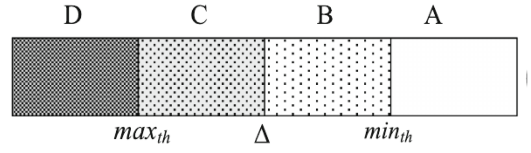
\includegraphics[scale=0.5]{static/images/queue_segments.png}
    \caption{Queue Segments}
    \label{fig:queue_segments}
\end{figure}


Just like traditional RED and its other variants, in FXRED, average queue length $avg$ is computed,

$$avg = (1-w)avg' + wq(t)$$

There are some other parameters that are used in the algorithm:

\begin{itemize}
  \item $\lambda(t)$: Total data arrival rate in the queue at time $t$.
  \item $\mu$: Bandwidth of the bottleneck link.
  \item $\rho(t)$: $\rho(t) = \lambda(t)/\mu$
\end{itemize}

Based on traffic load, three states are defined:

$$
  State-1: \rho(t) < 1, \\
  State-2: \rho(t) \approx 1,\\
  State-3: \rho(t) > 1. 
$$

\subsection*{\textbf{\texttt{Probability Function}}:}
$$
  p_d = \begin{cases}
        0 & avg < min_{th},\\
        2^{\lfloor k \rfloor}(\frac{avg-min_{th}}{max_{th}-min_{th}})^{\lfloor k\rfloor}.(1-\epsilon) & min_{th} \leq avg \lt \Delta, \\
        2\epsilon(\frac{avg-\Delta}{max_{th}-min_{th}}) + (1-\epsilon) & \Delta \leq avg \lt max_{th}, \\
        1 & avg \geq max_{th}
        \end{cases}
$$

$$
  k = c^{\frac{1}{\gamma}}, c \geq 2, 
  \epsilon = c^{-\gamma}
  \begin{cases}
        \gamma \lt 1 & State-1,
        \gamma \approx 1 & State-2,
        \gamma \geq c & State-3.
        \end{cases}
$$

\section*{Network Topologies Under Simulation}

\section*{\textbf{\texttt{1. Wired}}}
A dumbbell shaped topology is used where all the source nodes are connected to a single router and similarly all the destination nodes are connected to a single router. Both the routers are connected to each other through a link. The topology is shown below.

\begin{figure}
    \centering
    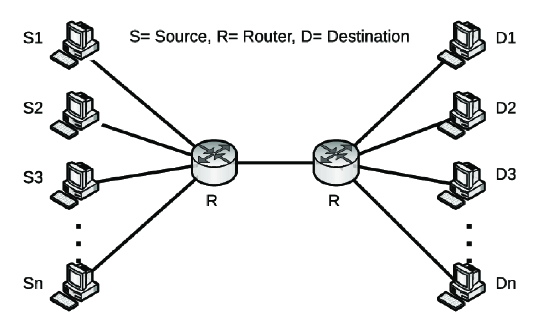
\includegraphics[scale=0.7]{static/images/wired_dumbbell_topology.png}
    \caption{Dumbbell Shaped Topology}
    \label{fig:dumbbell_topology}
\end{figure}


\section*{\textbf{\texttt{2. Wireless}}}
Nodes are randomly generated in a square area. For each simulation, a node is selected as source and a number of random nodes are selected as destination. Node configurations are as follows:

\begin{itemize}
  \item \texttt{Node Movement}: Static
  \item \texttt{Wireless MAC Type}: IEEE 802.15.4
  \item \texttt{Routing Protocol}: DSDV
  \item \texttt{Agent}: TCP
  \item \texttt{Application}: FTP
\end{itemize}

An example of the topology is shown below.

\begin{figure}[h]
    \centering
    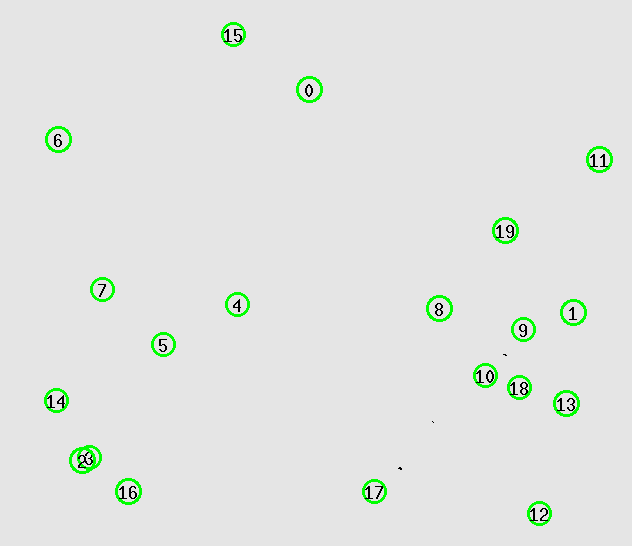
\includegraphics[scale=0.6]{static/images/wireless_topology.png}
    \caption{Wireless Topology}
    \label{fig:my_label}
\end{figure}

\section*{Parameters Under Variation}
To study the effect of different parameters on the performance of the network, the following parameters are varied in the simulation:

Base Parameters:

\begin{itemize}
  \item \texttt{Number of Nodes}: 20
  \item \texttt{Number of Flows}: 10
  \item \texttt{Packets Per Second}: 100
  \item \texttt{Coverage Area}: Tx\_Range = 250
\end{itemize}

Keeping one of the base parameters constant, the other parameters are varied in each simulation as follows:

\begin{itemize}
  \item \texttt{Number of Nodes}: 20, 40, 60, 80, 100
  \item \texttt{Number of Flows}: 10, 20, 30, 40, 50
  \item \texttt{Packets Per Second}: 100, 200, 300, 400, 500
  \item \texttt{Coverage Area}: Tx\_Range, 2x Tx\_Range, 3x Tx\_Range, 4x Tx\_Range, 5x Tx\_Range
\end{itemize}

\section*{Modifications in NS-2}
The following modifications are made in the NS-2 code to implement the FXRED algorithm:

Two files are changes in the \texttt{ns2.35/queue} directory:

\section*{\textbf{\texttt{red.h}}}
\begin{itemize}
  \item In \texttt{struct edp} the following two variables are added:
\begin{verbatim}
/*
* Parameters for FXRED
*/
double c; /* FXRED: constant c which should be greater than 2 */
int fxred; /* FXRED: enable/disable FXRED */
\end{verbatim}


  \item To keep track of the number of bytes arrived since the last time a packet was dropped, the following variables are added in \texttt{struct edv}
\begin{verbatim}
int count_bytes;		 /* # of bytes since last drop */
  double count_start_time; /* time when the count is 0 */
\end{verbatim}

Notice that the \texttt{count} variable is already there to keep track of the number of packets arrived since the last time a packet was dropped.

  \item A new method in \texttt{REDQueue:Queue} is added to calculate data arrival rate:
\begin{verbatim}
/*
* Calculate data arrival rate
*/
double getDataArrivalRate();
\end{verbatim}


\end{itemize}

\section*{\textbf{\texttt{red.cc}}}
Only the class \texttt{REDQueue} is modified. The following changes are made:

\begin{itemize}
  \item To pass parameter from tcl file to the class, the following code is added in \texttt{REDQueue::REDQueue()}:
\begin{verbatim}
bind("c_", &edp_.c);
bind_bool("fxred_", &edp_.fxred);
\end{verbatim}


  \item The two new parameters are initialized in \texttt{REDQueue::initparams()}:
\begin{verbatim}
edp_.fxred = 0;
edp_.c = 2.0;

edv_.count = 0;
edv_.count_bytes = 0;
\end{verbatim}


  \item In \texttt{REDQueue::reset()} just below the line \texttt{edv\_.count = 0;} the following line is added:
\begin{verbatim}
edv_.count_bytes = 0;
edv_.count_start_time = Scheduler::instance().clock();
\end{verbatim}

\textbf{These two lines are added everywhere where \texttt{edv\_.count = 0;} is present.}

  \item The \texttt{REDQueue::calculate\_p\_new()} is modified to calculate the probability function of FXRED.
\begin{verbatim}
double
REDQueue::calculate_p_new(double v_ave, double th_max, int gentle, 
double v_a, double v_b, double v_c, double v_d, double max_p)
{
  double p;

  if (edp_.fxred)
  {
    double miu = link_->bandwidth();
    double rho = getDataArrivalRate() / miu;
    double gamma = 1;
    double err = 0.01;
    double c = edp_.c;

    if (rho < 1.0 - err)
      gamma = 0.15;
    else if (rho > 1.0 + err)
      gamma = c;

    int k = pow(c, 1 / gamma);
    double epsilon = pow(c, -gamma);

    double th_min = edp_.th_min;
    double delta = (th_max + th_min) / 2;

    if (v_ave < th_min)
      p = 0.0;
    else if (th_min <= v_ave && v_ave < delta)
    {
      p = pow((v_ave - th_min) / delta, k);
      p *= 1 - epsilon;
    }
    else if (delta <= v_ave && v_ave < th_max)
    {
      p = 2 * epsilon * (v_ave - delta) / (th_max - th_min);
      p += 1 - epsilon;
    }
    else
      p = 1.0;
  }
  else
  {
    // default RED implementation
  }

  return p;
}
\end{verbatim}


  \item \texttt{REDQueue::modify\_p()}:
\begin{verbatim}
double
REDQueue::modify_p(double p, int count, int count_bytes, int bytes, 
  int mean_pktsize, int wait, int size)
{
  if (edp_.fxred)
  {
    p /= (1 - count * p);
  }
  else
  {
    // default RED implementation
  }
  return p;
}
\end{verbatim}

  \item Finally, the new definition of the function \texttt{REDQueue::getDataArrivalRate()} is added:
\begin{verbatim}
/*
* Calculates and returns the data arrival rate in bytes/sec.
*/
double REDQueue::getDataArrivalRate()
{
  double elapsed_time = Scheduler::instance().clock() - edv_.count_start_time;
  if (elapsed_time == 0.0)
    return 0;
    
  double rate = edv_.count_bytes / elapsed_time;
  return rate;
}
\end{verbatim}


\end{itemize}

\section*{Results with Graphs:}
% \textbf{\texttt{Wired}}
\section*{\textbf{\texttt{Wired}}}
Refer to the figures \ref{fig:wired_avg_delay}, \ref{fig:wired_del_ratio}, \ref{fig:wired_drp_ratio}, \ref{fig:wired_throughput} to see the outputs of wired topology.
\begin{figure}
    \centering
    \begin{subfigure}{.5\textwidth}
        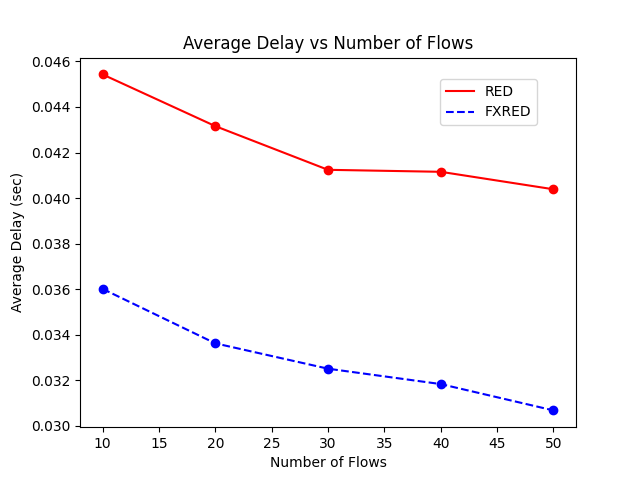
\includegraphics[width=1\linewidth]{static/graphs/wired/Average Delay vs Number of Flows.png}
    \end{subfigure}%
    \begin{subfigure}{.5\textwidth}
        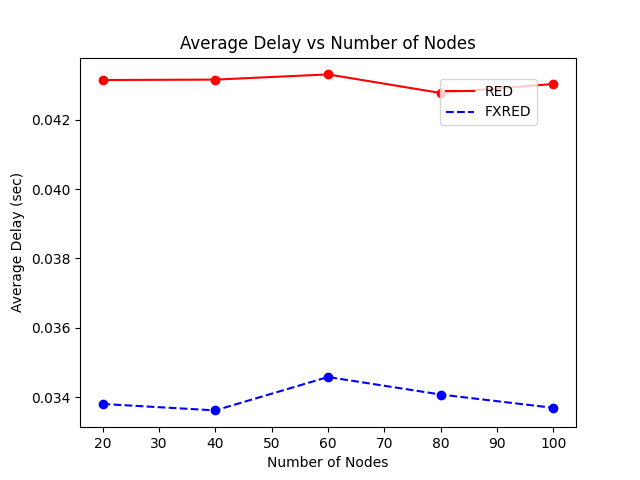
\includegraphics[width=1\linewidth]{static/graphs/wired/Average Delay vs Number of Nodes.png}
    \end{subfigure}

    \begin{subfigure}{.5\textwidth}
        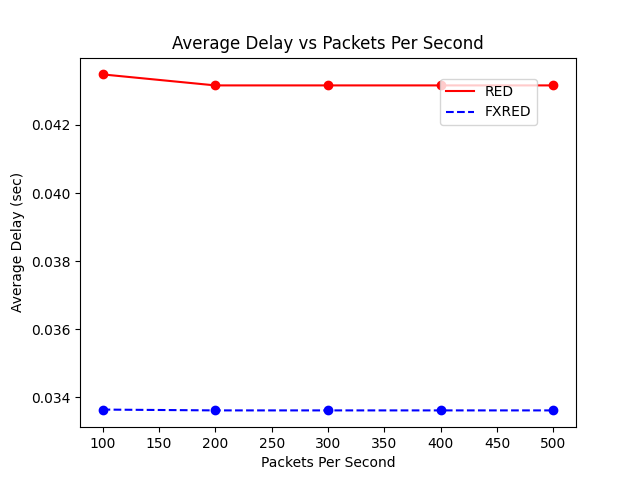
\includegraphics[width=1\linewidth]{static/graphs/wired/Average Delay vs Packets Per Second.png}
    \end{subfigure}
    \caption{Average Delay in Wired Topology}
    \label{fig:wired_avg_delay}
\end{figure}

\begin{figure}
    \centering
    \begin{subfigure}{.5\textwidth}
        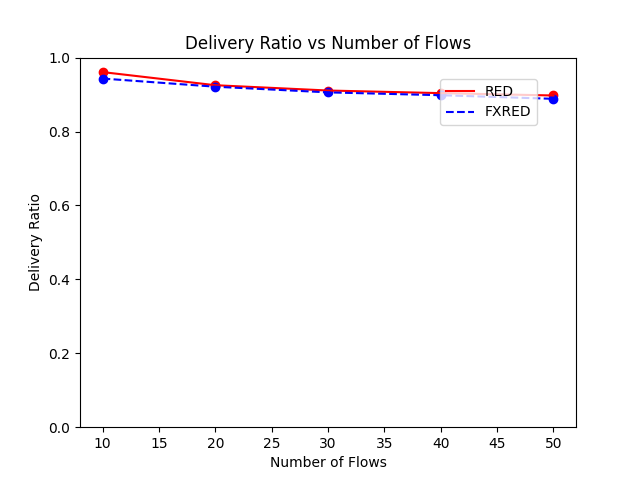
\includegraphics[width=1\linewidth]{static/graphs/wired/Delivery Ratio vs Number of Flows.png}
    \end{subfigure}%
    \begin{subfigure}{.5\textwidth}
        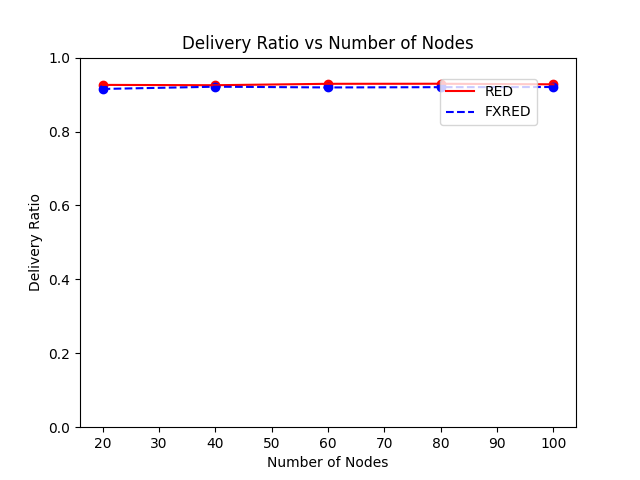
\includegraphics[width=1\linewidth]{static/graphs/wired/Delivery Ratio vs Number of Nodes.png}
    \end{subfigure}
    \begin{subfigure}{.5\textwidth}
        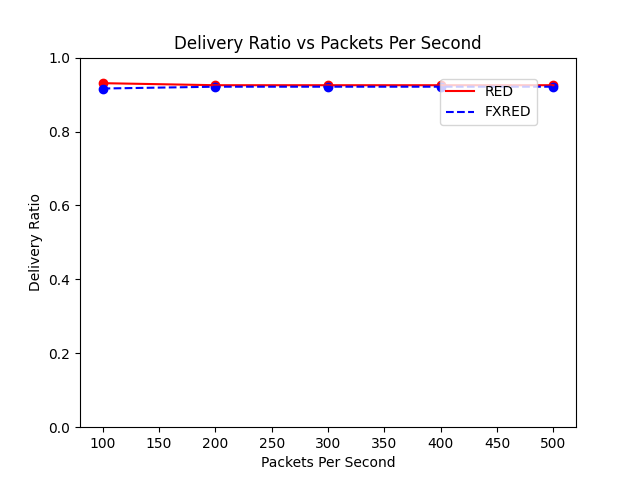
\includegraphics[width=1\linewidth]{static/graphs/wired/Delivery Ratio vs Packets Per Second.png}
    \end{subfigure}
    \caption{Delivery Ratio in Wired Topology}
    \label{fig:wired_del_ratio}
\end{figure}

\begin{figure}
    \centering
    \begin{subfigure}{.5\textwidth}
        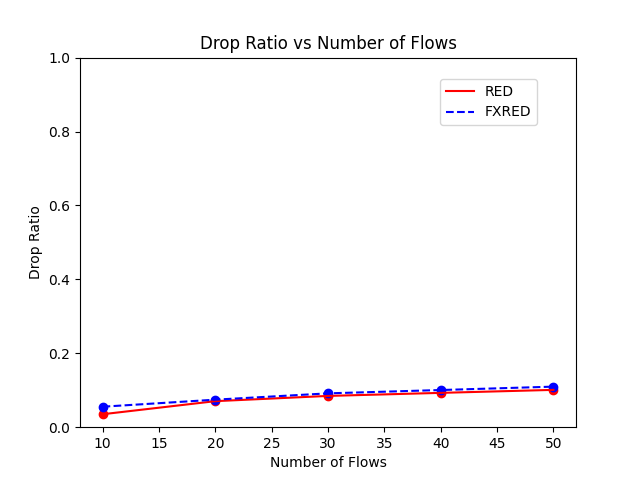
\includegraphics[width=1\linewidth]{static/graphs/wired/Drop Ratio vs Number of Flows.png}
    \end{subfigure}%
    \begin{subfigure}{.5\textwidth}
        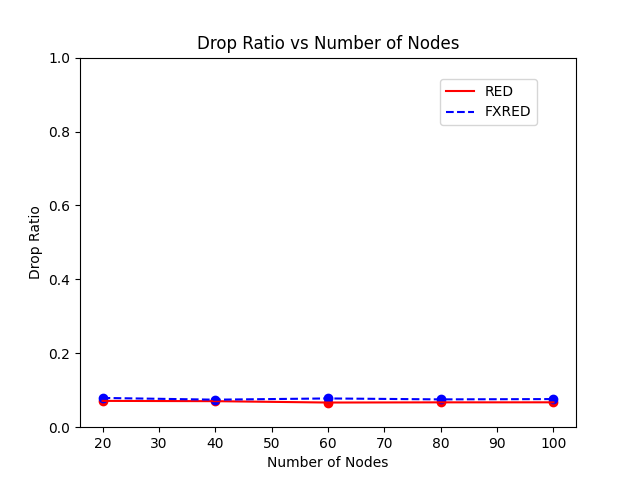
\includegraphics[width=1\linewidth]{static/graphs/wired/Drop Ratio vs Number of Nodes.png}
    \end{subfigure}

    \begin{subfigure}{.5\textwidth}
        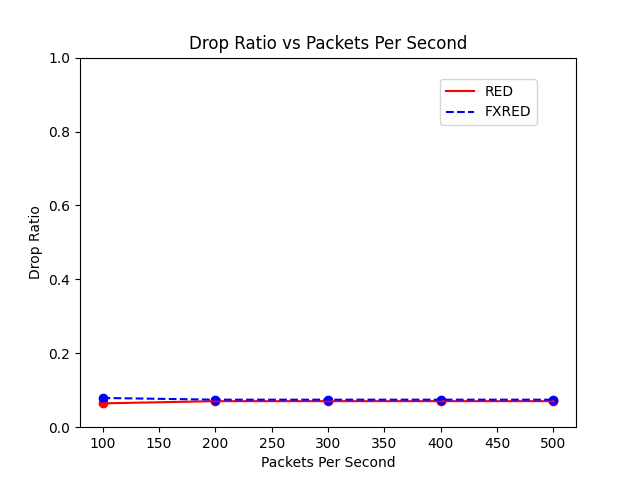
\includegraphics[width=1\linewidth]{static/graphs/wired/Drop Ratio vs Packets Per Second.png}
    \end{subfigure}
    \caption{Drop Ratio in Wired Topology}
    \label{fig:wired_drp_ratio}
\end{figure}

\begin{figure}
    \centering
    \begin{subfigure}{.5\textwidth}
        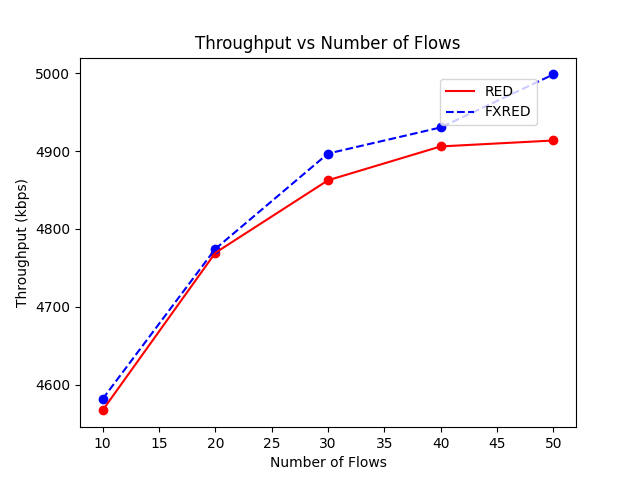
\includegraphics[width=1\linewidth]{static/graphs/wired/Throughput vs Number of Flows.png}
    \end{subfigure}%
    \begin{subfigure}{.5\textwidth}
        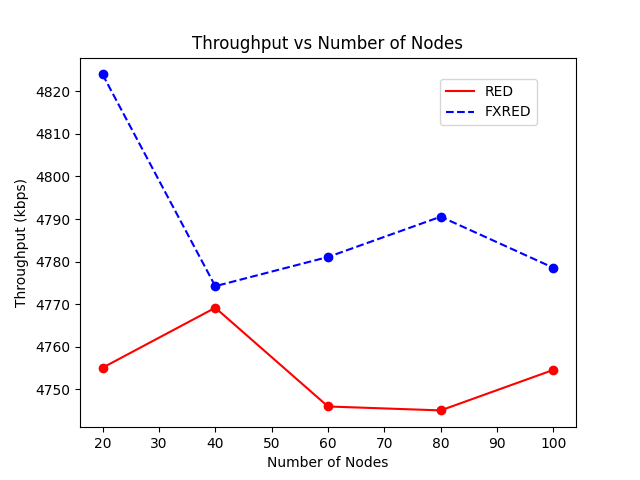
\includegraphics[width=1\linewidth]{static/graphs/wired/Throughput vs Number of Nodes.png}
    \end{subfigure}

    \begin{subfigure}{.5\textwidth}
        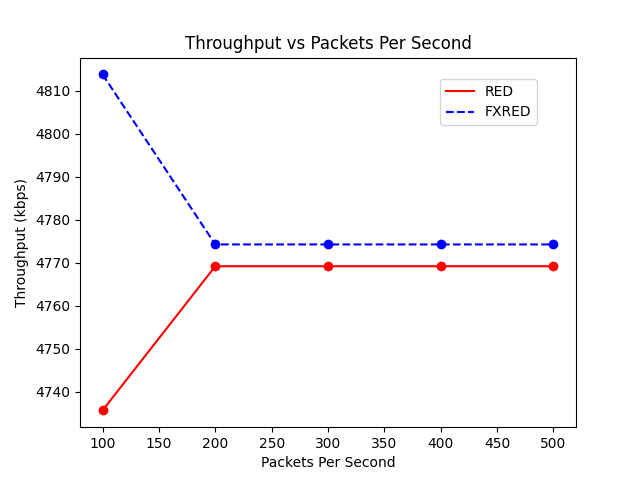
\includegraphics[width=1\linewidth]{static/graphs/wired/Throughput vs Packets Per Second.png}
    \end{subfigure}
    \caption{Throughput in Wired Topology}
    \label{fig:wired_throughput}
\end{figure}

\section*{\textbf{\texttt{Wireless}}}
Refer to the figures \ref{fig:wireless_avg_delay}, \ref{fig:wireless_del_ratio}, \ref{fig:wireless_drp_ratio}, \ref{fig:wireless_eng_consumption}, \ref{fig:wireless_throughput} to see the outputs of wireless topology.
\begin{figure}
    \centering
    \begin{subfigure}{.5\textwidth}
        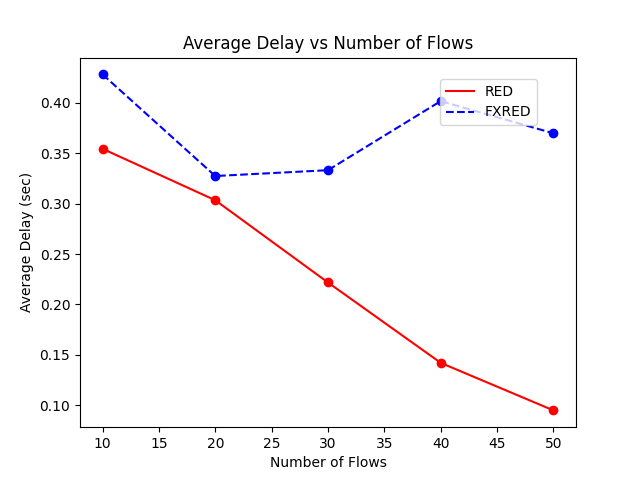
\includegraphics[width=1\linewidth]{static/graphs/wireless/Average Delay vs Number of Flows.png}
    \end{subfigure}%
    \begin{subfigure}{.5\textwidth}
        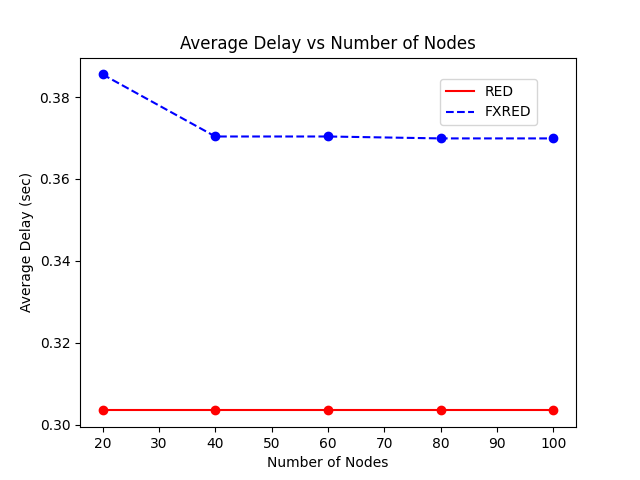
\includegraphics[width=1\linewidth]{static/graphs/wireless/Average Delay vs Number of Nodes.png}
    \end{subfigure}
    \begin{subfigure}{.5\textwidth}
        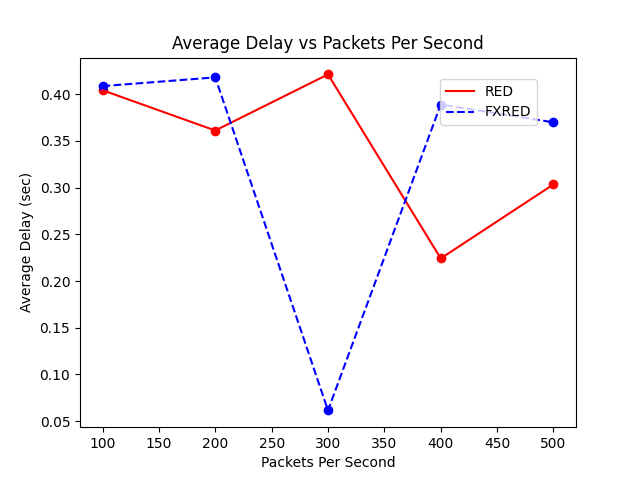
\includegraphics[width=1\linewidth]{static/graphs/wireless/Average Delay vs Packets Per Second.png}
    \end{subfigure}%
    \begin{subfigure}{.5\textwidth}
        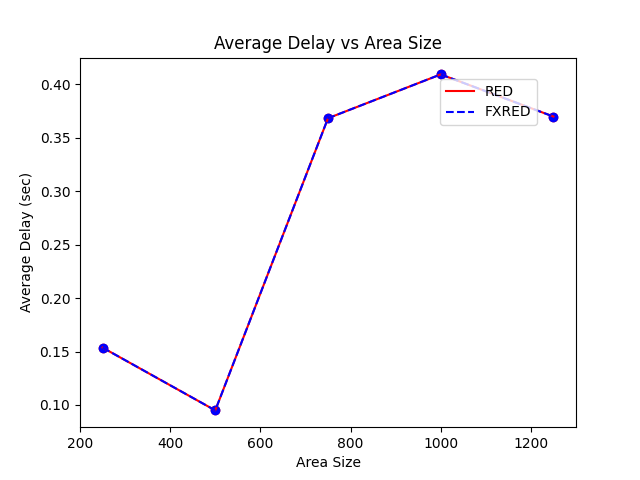
\includegraphics[width=1\linewidth]{static/graphs/wireless/Average Delay vs Area Size.png}
    \end{subfigure}
    \caption{Average Delay in Wireless Topology}
    \label{fig:wireless_avg_delay}
\end{figure}

\begin{figure}
    \centering
    \begin{subfigure}{.5\textwidth}
        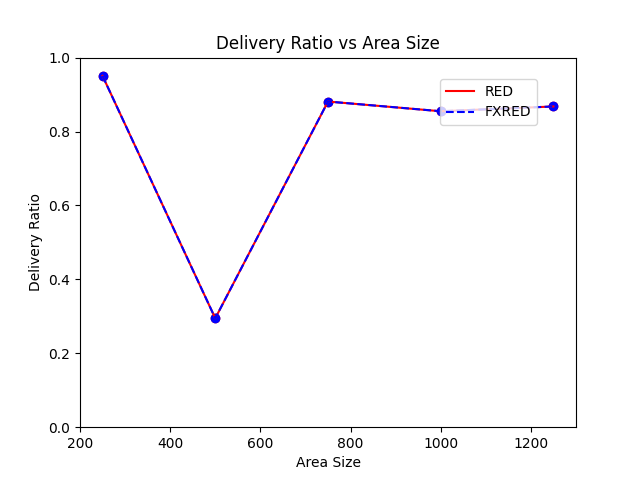
\includegraphics[width=1\linewidth]{static/graphs/wireless/Delivery Ratio vs Area Size.png}
    \end{subfigure}%
    \begin{subfigure}{.5\textwidth}
        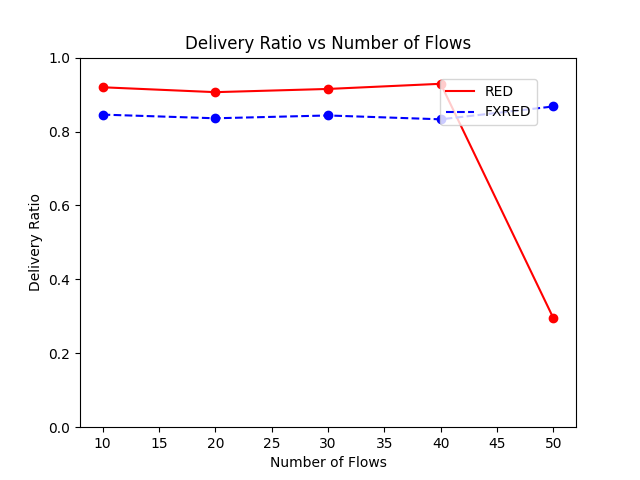
\includegraphics[width=1\linewidth]{static/graphs/wireless/Delivery Ratio vs Number of Flows.png}
    \end{subfigure}
    \begin{subfigure}{.5\textwidth}
        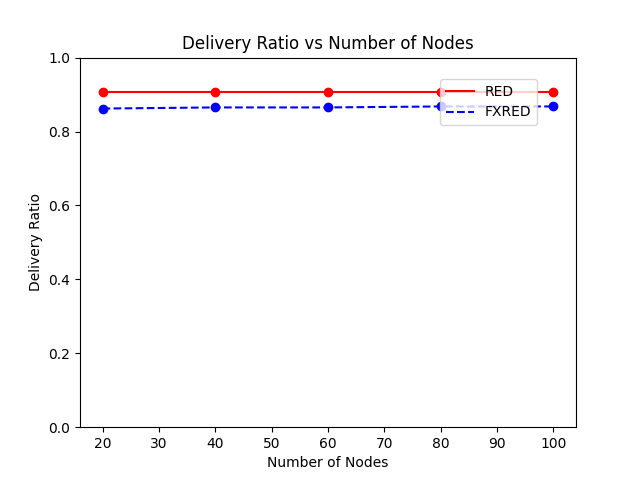
\includegraphics[width=1\linewidth]{static/graphs/wireless/Delivery Ratio vs Number of Nodes.png}
    \end{subfigure}%
    \begin{subfigure}{.5\textwidth}
        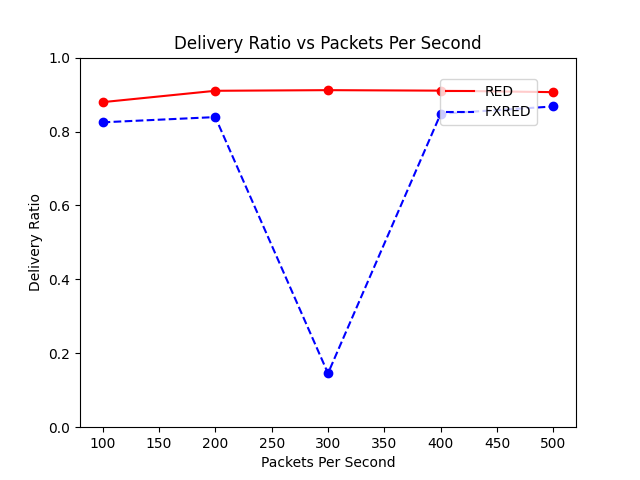
\includegraphics[width=1\linewidth]{static/graphs/wireless/Delivery Ratio vs Packets Per Second.png}
    \end{subfigure}
    \caption{Delivery Ratio in Wireless Topology}
    \label{fig:wireless_del_ratio}
\end{figure}

\begin{figure}
    \centering
    \begin{subfigure}{.5\textwidth}
        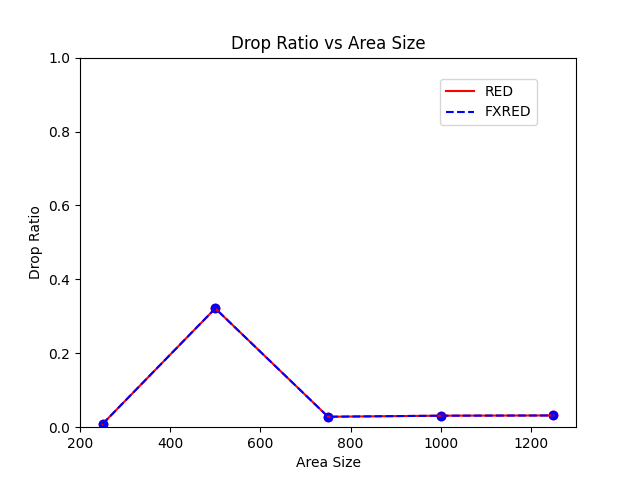
\includegraphics[width=1\linewidth]{static/graphs/wireless/Drop Ratio vs Area Size.png}
    \end{subfigure}%
    \begin{subfigure}{.5\textwidth}
        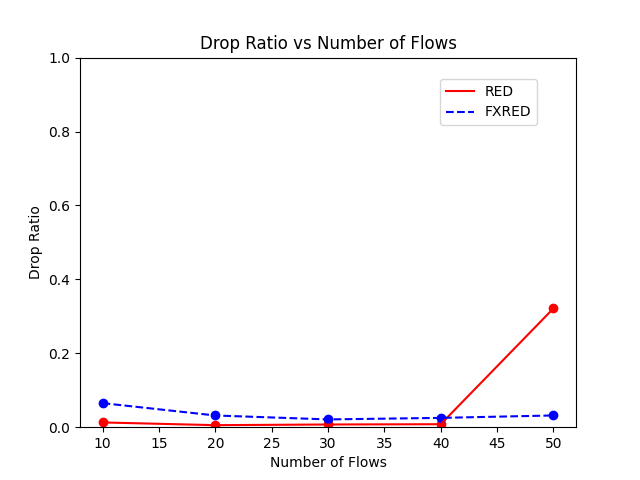
\includegraphics[width=1\linewidth]{static/graphs/wireless/Drop Ratio vs Number of Flows.png}
    \end{subfigure}
    \begin{subfigure}{.5\textwidth}
        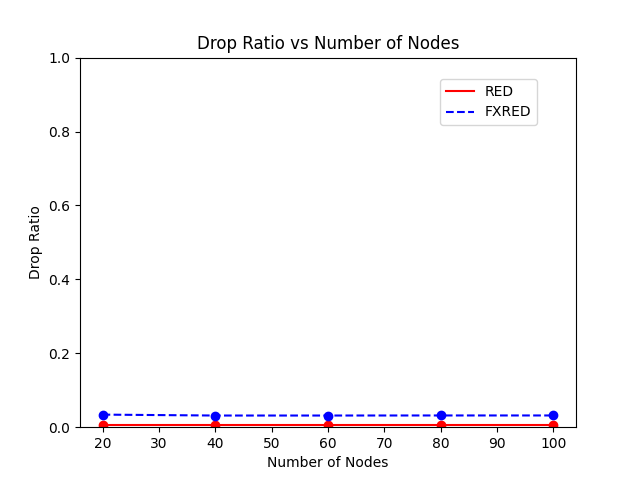
\includegraphics[width=1\linewidth]{static/graphs/wireless/Drop Ratio vs Number of Nodes.png}
    \end{subfigure}%
    \begin{subfigure}{.5\textwidth}
        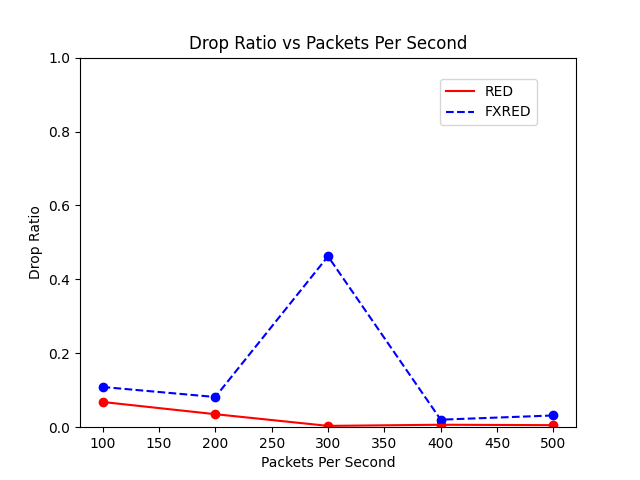
\includegraphics[width=1\linewidth]{static/graphs/wireless/Drop Ratio vs Packets Per Second.png}
    \end{subfigure}
    \caption{Drop Ratio in Wireless Topology}
    \label{fig:wireless_drp_ratio}
\end{figure}

\begin{figure}
    \centering
    \begin{subfigure}{.5\textwidth}
        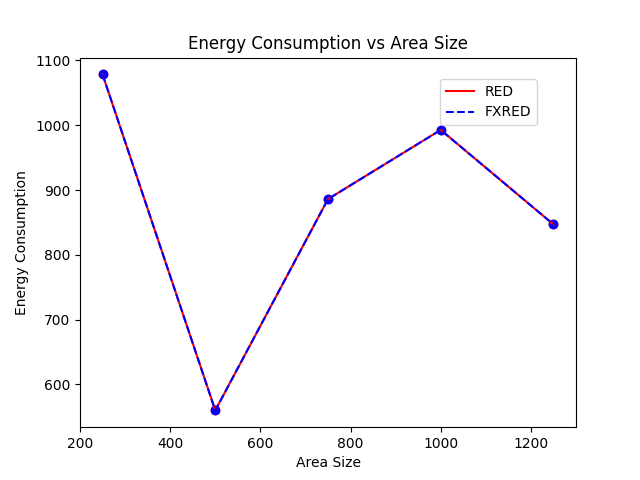
\includegraphics[width=1\linewidth]{static/graphs/wireless/Energy Consumption vs Area Size.png}
    \end{subfigure}%
    \begin{subfigure}{.5\textwidth}
        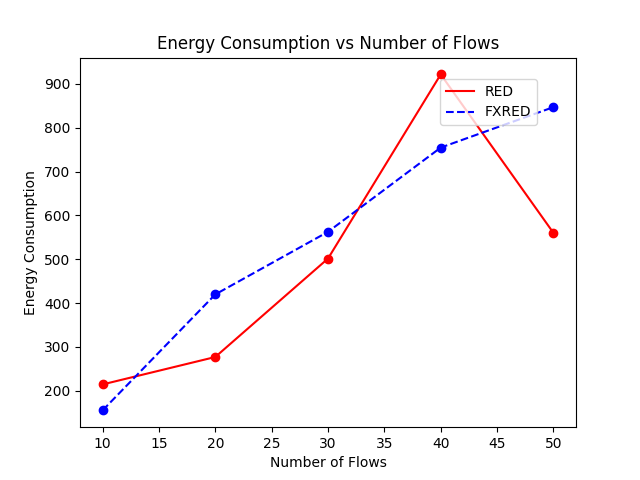
\includegraphics[width=1\linewidth]{static/graphs/wireless/Energy Consumption vs Number of Flows.png}
    \end{subfigure}
    \begin{subfigure}{.5\textwidth}
        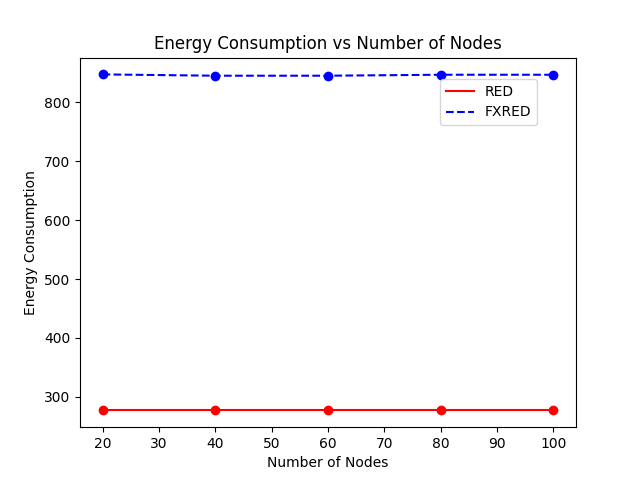
\includegraphics[width=1\linewidth]{static/graphs/wireless/Energy Consumption vs Number of Nodes.png}
    \end{subfigure}%
    \begin{subfigure}{.5\textwidth}
        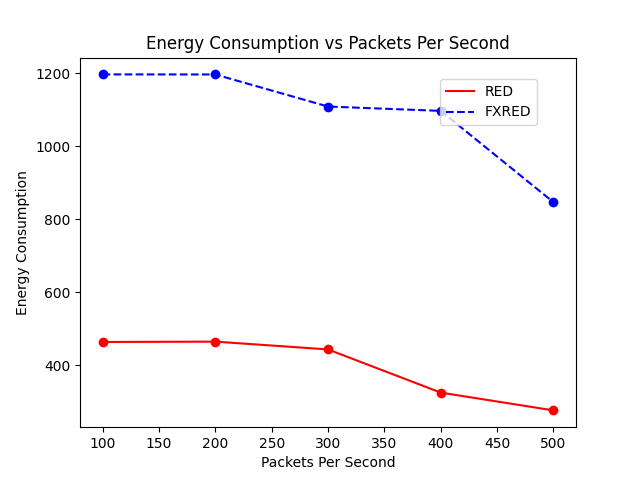
\includegraphics[width=1\linewidth]{static/graphs/wireless/Energy Consumption vs Packets Per Second.png}
    \end{subfigure}
    \caption{Energy Consumption in Wireless Topology}
    \label{fig:wireless_eng_consumption}
\end{figure}

\begin{figure}
    \centering
    \begin{subfigure}{.5\textwidth}
        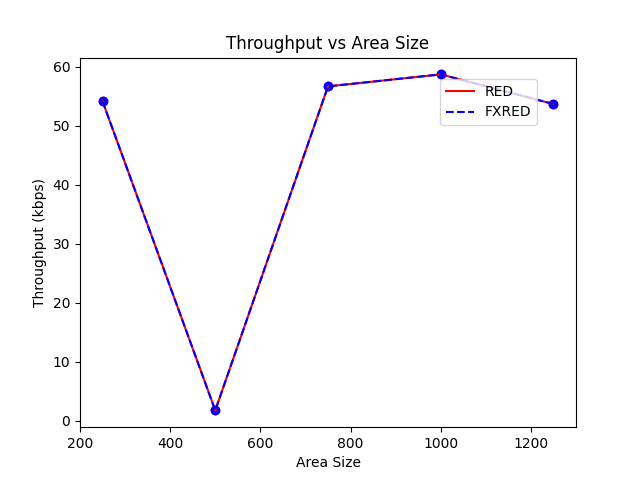
\includegraphics[width=1\linewidth]{static/graphs/wireless/Throughput vs Area Size.png}
    \end{subfigure}%
    \begin{subfigure}{.5\textwidth}
        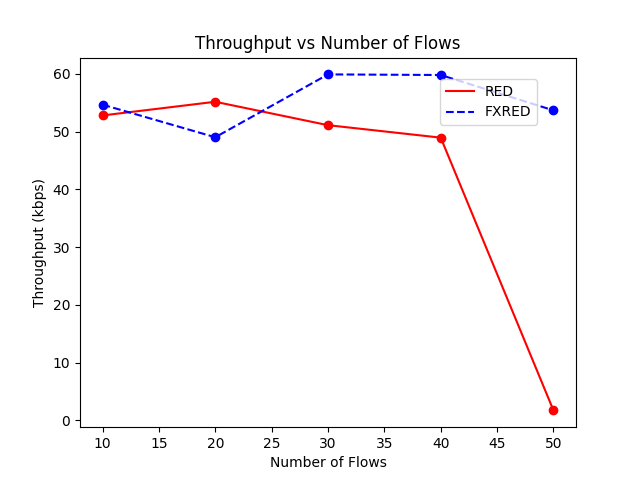
\includegraphics[width=1\linewidth]{static/graphs/wireless/Throughput vs Number of Flows.png}
    \end{subfigure}
    \begin{subfigure}{.5\textwidth}
        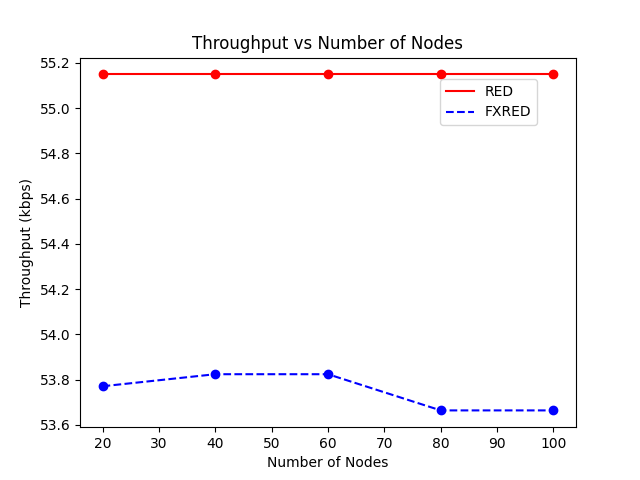
\includegraphics[width=1\linewidth]{static/graphs/wireless/Throughput vs Number of Nodes.png}
    \end{subfigure}%
    \begin{subfigure}{.5\textwidth}
        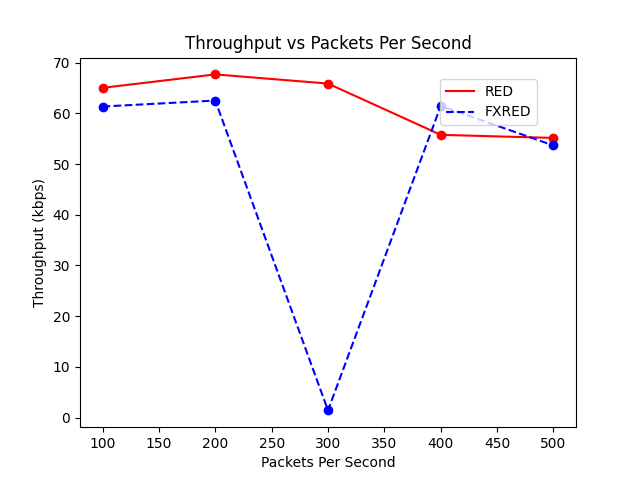
\includegraphics[width=1\linewidth]{static/graphs/wireless/Throughput vs Packets Per Second.png}
    \end{subfigure}
    \caption{Throughput in Wireless Topology}
    \label{fig:wireless_throughput}
\end{figure}

\section*{Summary of Findings:}
From the graphs found after analysing wired topology, we can see that the proposed algorithm works better in terms of end to end average delay but it has a higher drop ratio. This is because the proposed algorithm is more aggressive in dropping packets. The proposed algorithm also has a higher throughput than the default RED algorithm. In terms of delivery ratio, both algorithms have a similar performance.

On the other hand, wireless topology suggests quite a different result. The proposed algorithm has a higher end to end average delay than the default RED algorithm. Delivery ratio and throughput are also lower in FXRED. Drop ratio and energy consumption are slightly higher too.

\section*{Conclusion:}
As we use RED algorithms to control congestion, the dumbbell shaped wired topology is more suitable for simulating the performance of RED algorithms. So, we can rely on the results found in wired topology to conclude that the proposed algorithm is slightly better than the default RED algorithm.

\bibliographystyle{plain}
\bibliography{bibs/fxred_paper}

\end{document}


    